\documentclass{article}

%\usepackage{fullpage}
\usepackage{graphicx}
\usepackage{color}
\usepackage{amsmath}
\usepackage{amssymb}

\newcommand{\trace}{\mathrm{trace}}
\newcommand{\diag}{\mathrm{diag}}
\newcommand{\sspan}{\mathrm{span}}
\newcommand{\sfC}{\mathsf{C}}
\newcommand{\bfI}{\mathbf{I}}
\newcommand{\um}{\ensuremath{\mu m}}
\newcommand{\calK}{\ensuremath{\mathcal{K}}}
\newcommand{\Kdynamic}{\ensuremath{K_{\mathrm{dyn}}}}
\newcommand{\Lambdaip}{\left( \Lambda^{-1} \right)}
\renewcommand{\Re}{\mathrm{Re}}
\renewcommand{\Im}{\mathrm{Im}}

\newcommand{\note}[1]{\footnote{\textsc{To do}: #1}}


\title{Elastic PMLs for resonator loss simulation}
\author{David Bindel}

\begin{document}

\maketitle

\begin{abstract}
  High frequency electromechanical resonators are used in frequency
  references, filters, and sensors.  Surface-micromachined
  MEMS resonators are an attractive alternative to existing quartz,
  ceramic, and SAW devices; but to be viable, these MEMS resonators must
  have a very high quality of resonance ($Q$).  Depending on scale and
  geometry, the energy losses that lower $Q$ may primarily come from
  material damping, thermoelastic damping, air damping, or radiation of
  elastic waves from an anchor.  In this report, we describe how
  anchor losses can be computed using an absorbing boundary
  based on a \emph{perfectly matched layer} (PML) which absorbs
  incoming waves over wide frequency range for any non-zero angle of
  incidence.  We show how to interpret the PML as a complex-valued
  change of coordinates, and illustrate how this interpretation leads
  to a simple finite element implementation.  As an example application,
  we compute the anchor loss in a model of a MEMS disk resonator.
  Our analysis illustrates a surprising mode-mixing phenomenon which can
  substantially affect the quality of resonance.
\end{abstract}


\section{Introduction}

Modern communication systems rely on high-frequency electromechanical
resonators to act as frequency references and filters.  Though
designers currently use quartz, ceramic, and surface-acoustic wave
devices, surface-micromachined MEMS resonators in development offer an
attractive alternative.  Because they can be integrated into CMOS,
MEMS resonators have the potential to cost less area, power, and money
than existing alternatives~\cite{Nguyen:2001:VRM}.  But to be viable,
energy losses in these MEMS resonators must be minimized.  The usual
measure of this energy loss is the \emph{quality factor} $Q$ of a
resonant peak, defined as
\begin{equation}
  \label{Q-def}
  Q = 2 \pi \left(
      \frac{\mbox{Stored energy}}
           {\mbox{Energy lost per period}}
      \right).
\end{equation}
Resonators in cell phone filters require $Q$ values greater than 1000
for good performance, and higher values are 
preferable~\cite{Nguyen:2001:VRM,Aigner:2003:RFM}.

Depending on scale, geometry, and materials, the energy losses that
lower $Q$ may come from material damping, air damping, thermoelastic
damping, or radiation of elastic waves from an
anchor~\cite{Candler:2003:IEL}.  While losses in low-frequency
resonators are dominated by air damping, for which increasingly
accurate compact models are available~\cite{Ye:2003:ADL,Bao:2003:MRE},
very high-frequency disk resonators have similar measured performance
in vacuum or air~\cite{Wang:2003:SAG}.  Thermoelastic damping is a
frequently-cited source of losses at high
frequencies~\cite{Duwel:2003:EST,Houston:2002:TLM,Abdolvand:2003:TDT,Lifshitz:2000:TDM,Srikar:2002:TDF}.
In most cases, the damping is estimated by fitting parameters in a
model originally developed by
Zener~\cite{Zener:1937:IFS,Zener:1938:IFSa,Zener:1938:IFSb};
unfortunately, this parameter-fitting makes it difficult to tell what
should be attributed to thermoelastic effects and what should be
attributed to other sources of damping with similar functional form.
Though anchor damping is a recognized source of
losses~\cite{Candler:2003:IEL}, there are relatively few MEMS papers
(see e.g.~\cite{Park:2004:HFMa,Park:2004:HFMb}) dealing with losses at
the anchor.

Although it is not well studied, in several designs for high MHz or
GHz frequency resonators, the dominant loss mechanism appears to be
radiation of elastic energy through anchors.  In these designs, the
resonating device is so much smaller than the silicon substrate on
which it sits that waves radiating from the anchor are sufficiently
attenuated by material losses that reflections from the sides of the
chip toward the anchor are negligible.  That is, the bulk of the chip
can effectively be modeled as a semi-infinite medium.  We model this
semi-infinite domain using a \emph{perfectly matched layer} (PML),
which absorbs waves from any angle of incidence~\cite{Basu:2003:PML}.
We describe the PML and its interpretation in detail, and also show
how to construct reduced-order models which preserve the structure of
the PML equations.

To illustrate the PML technology, we analyze the behavior of a family
of MEMS disk resonators.  Several variants of this design have already
been fabricated~\cite{Wang:2003:SAG,Wang:2004:GND}, and illustrate $Q$
as high as $55000$ at $1.14$ GHz.  Through our numerical experiments,
we show how energy is lost to the substrate through a ``pumping''
mechanism, in which the predominantly horizontal motion of the disk
drives is converted into vertical motion at the post through the
Poisson effect.  We also show how, near critical values for the
geometric parameters, the mixing of two modes can lead to dramatic
variation in the value of $Q$.


\section{Perfectly matched layers}
\label{pml-section}

Except for scale, a microresonator atop a silicon chip is much like a
structure on the earth's surface during an earthquake.  While we are
concerned with waves radiating away from a structure and the
earthquake engineer is concerned with waves radiating toward a
structure, in both cases the substrate is much larger than the
structure, and it can be modeled as an elastic half-space.  This
infinite-domain approximation occur in many physical models: acoustic
waves radiating from a musical instrument, electromagnetic waves
reflecting from aircraft, elastic waves scattering from a crack in a
solid, and water waves in an open harbor are only a few additional
examples~\cite{Turkel:1998:ISI,Zienkiewicz:2000:FEMc}.  The essential
characteristic of the infinite-domain solution is that only outgoing
waves are allowed.  To model infinite-domain problems on a computer,
we need finite-size discretizations which enforce this radiation
condition.

One way to enforce the radiation condition is to discretize an exact
boundary equation satisfied by outgoing waves.  For example, outside
of a sphere containing any radiators and scatterers, waves can be
written as a multipole expansion; in this expansion, the radiation
condition just says that certain coefficients corresponding to
incoming waves should be zero.  A related global condition is the DtN
map, which specifies how Dirichlet conditions and Neumann conditions
must be related at a surface~\cite{Turkel:1998:ISI}.  These boundary
conditions are rigorously derived and highly accurate, but they
usually require that the artificial boundary have a particular shape.
They are also nonlocal in space: every boundary unknown is directly
related to every other boundary unknown, and consequently the matrix
of boundary terms is dense, and expensive to form and to solve.
Furthermore, exact boundary conditions may be unavailable for problems
in which no analytically tractable Green's function is known, as in
the case of an elastic half space.

An alternative approach is to build approximate boundary conditions
based on the asymptotic behavior of outgoing waves.  These approximate
conditions are local and inexpensive, but only absorb waves over a
small range of angles of
incidence~\cite{Turkel:1998:ISI,Basu:2003:PML}.  Consequently, a large
computational domain may be needed for accurate results.  Yet another
approach is to add a nonphysical ``sponge layer'' to dissipate waves
before they reach the artificial boundary.  Waves passing through the
sponge layer are damped on the way to the artificial boundary, and are
further damped when they are reflected back, so that most of the
signal entering the layer is absorbed.  To be effective, though, the
layer must be designed so that there is no impedance mismatch to
reflect waves back from the interface between the layer and the rest
of the domain.

A \emph{perfectly matched layer} (PML) is a refinement of a sponge
layer.  B{\'e}renger invented the perfectly matched layer for problems
in electromagnetic wave propagation~\cite{Berenger:1994:PML}, and it
was later re-interpreted as a complex-valued change of coordinates
which could be applied to any linear wave
equation~\cite{Turkel:1998:APB,Teixeira:2000:CSA}.  Not only do these
layers rapidly attenuate waves, but they also ``perfectly match'' the
rest of the domain; that is, there are no spurious reflections at the
interface.  We describe an alternate interpretation of a perfectly
matched layer for time-harmonic elastodynamics which was described
in~\cite{Basu:2003:PML}, and show how our interpretation leads to a
simple finite element implementation.



\subsection{A motivating example}

Consider a longitudinal wave propagating down a homogeneous,
semi-infinite rod with axial coordinate $x \in [0, \infty)$.  If waves
travel with speed $c$, the one-dimensional wave equation that
describes this system is
\begin{equation}
  \frac{d^2 u}{dx^2} - \frac{1}{c^2} \frac{d^2 u}{dt^2} = 0
\end{equation}
where $u(x,t)$ is the displacement.
\note{
  Do I want to cover evanescent waves, too?
}
Time-harmonic solutions $u(x,t) = \hat{u}(x) e^{i \omega t}$
are governed by a Helmholtz equation
\begin{equation}
  \label{helmholtz-eq-1d}
  \frac{d^2 \hat{u}}{dx^2} + k^2 \hat{u} = 0.
\end{equation}
where $k = \omega/c$ is the wave number.  Solutions to this problem
have the form
\begin{equation}
  \hat{u} = c_{\mathrm{out}} e^{-ikx} + c_{\mathrm{in}} e^{ikx}
\end{equation}
where $c_{\mathrm{out}}$ is the magnitude of the outgoing wave traveling
from the origin toward infinity, and $c_{\mathrm{in}}$ is the magnitude
of the incoming wave traveling from infinity toward the origin.
In general, we assume there is no source at infinity, so physically meaningful
solutions to the problem have $c_{\mathrm{in}} = 0$.

We now consider the same equation under a change of coordinates.  Let
$\lambda(s)$ be a continuous, complex-valued function which is nowhere
zero, and define a new coordinate
\begin{equation}
  \tilde{x} = \int_0^x \lambda(s) \, ds.
\end{equation}
By definition, $\tilde{x}$ and $x$ are differentially related
\begin{equation}
  \frac{d \tilde{x}}{dx} = \lambda(x) 
  \hspace{1cm}
  \frac{d}{d \tilde{x}} = \frac{1}{\lambda(x)} \frac{d}{dx}.
\end{equation}
Now suppose that that the stretched coordinate $\tilde{x}$ is used
as the independent variable in equation (\ref{helmholtz-eq-1d}).
Then in terms of $x$, the equation is
\begin{equation}
  \label{pml-eq}
  \frac{1}{\lambda} \frac{d}{dx} 
    \left( \frac{1}{\lambda} \frac{d\hat{u}}{dx} \right) +
  k^2 \hat{u} = 0.
\end{equation}
where the derivative may be taken in a weak sense, since $\lambda$
need not be $C^1$.
Equation (\ref{pml-eq}) describes wave propagation in a
\emph{perfectly matched medium} (PMM).  While it is motivated by a complex
coordinate-stretch, the perfectly matched medium may be defined
independent of $\tilde{x}$.

\begin{figure}
  \begin{center} \scalebox{0.7}{ \begin{picture}(0,0)
\ifx\pdfoutput\undefined
  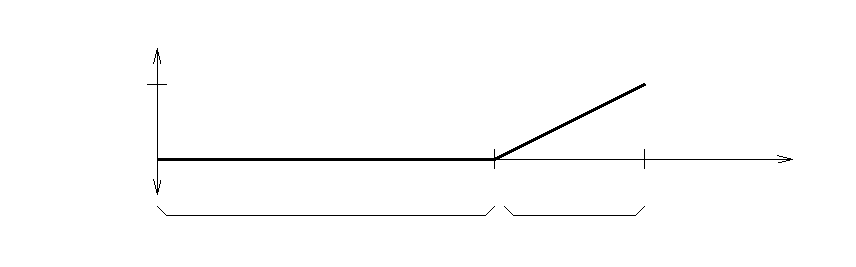
\includegraphics{attenuate.ps}
\else
  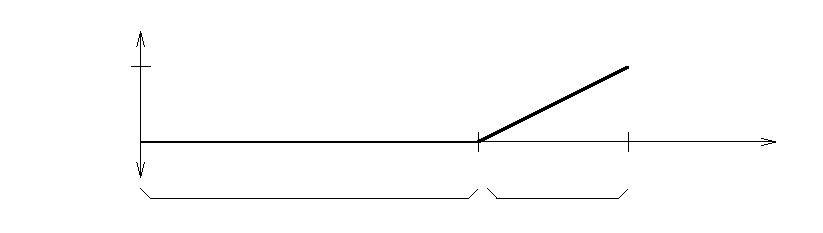
\includegraphics{attenuate.pdf}
\fi
\end{picture}
\setlength{\unitlength}{3947sp}%
%
\begingroup\makeatletter\ifx\SetFigFont\undefined%
\gdef\SetFigFont#1#2#3#4#5{%
  \reset@font\fontsize{#1}{#2pt}%
  \fontfamily{#3}\fontseries{#4}\fontshape{#5}%
  \selectfont}%
\fi\endgroup%
\begin{picture}(6576,1860)(-824,-1090)
\put(226,614){\makebox(0,0)[lb]{\smash{{\SetFigFont{12}{14.4}{\familydefault}{\mddefault}{\updefault}{\color[rgb]{0,0,0}$\sigma$}%
}}}}
\put(601,-1036){\makebox(0,0)[lb]{\smash{{\SetFigFont{12}{14.4}{\familydefault}{\mddefault}{\updefault}{\color[rgb]{0,0,0}Bounded domain}%
}}}}
\put(5476,-436){\makebox(0,0)[lb]{\smash{{\SetFigFont{12}{14.4}{\familydefault}{\mddefault}{\updefault}{\color[rgb]{0,0,0}$x$}%
}}}}
\put(2851,-661){\makebox(0,0)[lb]{\smash{{\SetFigFont{12}{14.4}{\familydefault}{\mddefault}{\updefault}{\color[rgb]{0,0,0}$L$}%
}}}}
\put(3976,-661){\makebox(0,0)[lb]{\smash{{\SetFigFont{12}{14.4}{\familydefault}{\mddefault}{\updefault}{\color[rgb]{0,0,0}$L_p$}%
}}}}
\put(3076,-1036){\makebox(0,0)[lb]{\smash{{\SetFigFont{12}{14.4}{\familydefault}{\mddefault}{\updefault}{\color[rgb]{0,0,0}PML region}%
}}}}
\put(-824,164){\makebox(0,0)[lb]{\smash{{\SetFigFont{12}{14.4}{\familydefault}{\mddefault}{\updefault}{\color[rgb]{0,0,0}$\beta (L_p-L)$}%
}}}}
\end{picture}%
 } \end{center}
  \vspace{-3mm}
  \caption{Piecewise linear attenuation function for a plane wave}
  \label{sigma-schematic}
\end{figure}

Suppose
\begin{equation}
 \label{lambda-helmholtz-def}
 \lambda(s) = 1 - i \sigma(s) / k; 
\end{equation}
then the solutions to 
the PMM equation (\ref{pml-eq}) are
\begin{eqnarray}
  \hat{u} = 
    c_{\mathrm{out}} \exp\left(-\int_0^x \sigma(s) \, ds \right) 
                     \exp\left( -i k x \right) +
    c_{\mathrm{in}} \exp\left(\int_0^x \sigma(s) \, ds \right) 
                     \exp\left( i k x \right).
\end{eqnarray}
So long as $\sigma = 0$, both the incoming and outgoing solutions to
the PMM equation (\ref{pml-eq}) agree with the solutions to the
original Helmholtz equation (\ref{helmholtz-eq-1d}).  Where $\sigma >
0$, the wave decays in the direction of travel.  Since the outgoing
wave and the incoming wave travel in opposite directions, the outgoing
wave amplitude decays with $x$, while the incoming wave amplitude
grows with $x$.  For example, suppose $\sigma$ is defined to be zero
on $[0,L]$ and $\sigma = \beta (s-L)$ on $[L,\infty)$
(Figure~\ref{sigma-schematic}).  Then for $x > L$, the outgoing wave
amplitude is $c_\mathrm{out} \exp\left( -\beta(x-L)^2/2 \right).$ The
incoming wave grows at the same rapid rate that the outgoing wave
decays.  Therefore, an appropriate replacement for Sommerfeld's
radiation condition for the original problem is that solutions should
decay to zero as $x \rightarrow \infty$.
%\note{
%  Sanjay's comment: State clearly from the outset that the wave decays
%  in the direction of travel.  Also, give the anisotropic medium
%  interpretation for the scalar wave equation, and explain why it doesn't
%  carry over to ordinary elasticity.
%}

Because waves decay so rapidly as they travel through the PML region,
we get a good approximation to the infinite-domain problem even if we
force $\hat{u}(L_p) = 0$ for some finite $L_p > L$.  For example,
suppose we prescribe $\hat{u}(0) = 1$ and $\hat{u}(L_p) = 0$.  For
convenience, define $\gamma = \beta(L_p-L)^2$; then the boundary
conditions become
\begin{equation}
  \begin{bmatrix}
    \hat{u}(0) \\ \hat{u}(L_p)
  \end{bmatrix} =
  \begin{bmatrix}
    1 & 1 \\
    e^{-(\gamma/2 + ikL_p)} & e^{\gamma/2 + ikL_p}
  \end{bmatrix}
  \begin{bmatrix}
    c_\mathrm{out} \\ c_\mathrm{in}
  \end{bmatrix} =
  \begin{bmatrix} 1 \\ 0 \end{bmatrix}
\end{equation}
and therefore
\begin{equation}
  c_\mathrm{out} = \frac{1}{1 - e^{-\gamma-2ikL_p}} 
                 = 1 + O(e^{-\gamma})
\hspace{1cm}
  c_\mathrm{in} = \frac{-e^{-\gamma-2ikL_p}}{1 - e^{-\gamma-2ikL_p}}
                = -O(e^{-\gamma}).
\end{equation}
Even for modest $\gamma$, the bounded-domain solution is a good
approximation to the infinite domain solution.  For $\gamma \approx
4.6$, only 1\% of the outgoing wave is reflected.
Increasing $\gamma$ decreases the reflection in the continuous case; 
if $\gamma$ is too large, though, the solution can decay so quickly that
many points in the PML are needed to obtain an accurate discretization.
\note{
  Can I do a 1-D analysis to quantify that last statement?
}


\subsection{Elastic perfectly matched layers}
\label{elastic-pml-section}

The equations of motion for a time-harmonic elastodynamic medium with
no body forces are
\begin{eqnarray}
  \omega^2 \rho u + \nabla \cdot \sigma & = & 0 \label{strong-form-eq} \\
  \sigma & = & \sfC \epsilon 
    \label{linear-stress-strain-eq} \\
  \epsilon & = & \left( \frac{\partial u}{\partial x} \right)^s
\end{eqnarray}
where $u$ is the displacement field, $\epsilon$ is the infinitesimal
strain tensor, $\sigma$ is the stress tensor, $\sfC$ is the material
stiffness tensor, and $\rho$ is the density.  A simple isotropic
elastic medium admits propagating disturbances moving at two characteristic
velocities: there are faster-moving compression waves ($P$ waves), and
slower-moving shear waves ($S$ waves).  An anisotropic medium admits
even more characteristic wave speeds, and inhomogeneities and interfaces
add yet more wave types.
%Various types of interface-guided
%waves are also possible.
%\note{
%  Single-crystal Si and the various piezo crystal films are anisotropic --
%  better say something about that case, too.
%}
As in the one-dimensional case, though,
a complex coordinate transformation can be used to attenuate each
of these waves in the direction of travel without spurious reflections
from artificial interfaces.
\note{
  I think I may be able to refine Ushnish's analysis by either
  introducing modified scalar and vector potentials, or by tracing the
  behavior along characteristics.
}

Though it is possible to introduce the coordinate transformation into
the local form of the equations, it is simpler to recast the equations
in weak form and then transform.  The weak form of the time-harmonic
elastodynamic equation is
\begin{equation}
  \int_\Omega \epsilon(w) : \sigma(u) \, d\Omega -
  \omega^2 \int_\Omega \rho w \cdot u \, d\Omega =
  \int_{\Gamma} w \cdot t \, d\Gamma 
  \label{weak-form-eq}
\end{equation}
where the domain is $\Omega$, part of the boundary $\Gamma \subset
\partial \Omega$ is subject to tractions $t$, and $w$ is a weight
function.  As before, suppose $\tilde{x}$ is a transformed coordinate
such that the Jacobian $\frac{\partial \tilde{x}}{\partial x} =
\Lambda$ is continuously defined and everywhere nonsingular.
Replacing $x$ with $\tilde{x}$ in (\ref{weak-form-eq}), we have
\begin{equation}
  \int_{\tilde{\Omega}}
    \tilde{\epsilon}(w) : \tilde{\sigma}(u) \, d\tilde{\Omega} -
  \omega^2 \int_{\tilde{\Omega}} \rho w \cdot u \, d\tilde{\Omega} =
  \int_{\tilde{\Gamma}} 
    w \cdot \tilde{\sigma}(u) \cdot \tilde{n} d\tilde{\Gamma}
  \label{weak-form-eq2}
\end{equation}
We now map back to the $x$ coordinate system:
\begin{equation}
  \int_{\Omega} 
    \tilde{\epsilon}(w) : \tilde{\sigma}(u) \, \det(\Lambda) d\Omega -
  \omega^2 \int_\Omega \rho w \cdot u \, \det(\Lambda) d\Omega =
  \int_{\Gamma}
    w \cdot \tilde{\sigma}(u) \cdot (\Lambda^{-T} n) \det(\Lambda) \, d\Gamma.
  \label{weak-form-eq3}
\end{equation}
In the $x$ coordinate system, the transformed strain and stress tensors are
\begin{eqnarray}
  \tilde{\epsilon}(u) 
   & = & \left( \frac{\partial u}{\partial \tilde{x}} \right)^s
     =   \left( \frac{\partial u}{\partial x} \Lambda^{-1} \right)^s \\
  \tilde{\sigma}(u)
   & = & \sfC \tilde{\epsilon}(u).
\end{eqnarray}
The local form of (\ref{weak-form-eq3}), which can be derived either
from (\ref{weak-form-eq3}) or directly from transforming 
(\ref{strong-form-eq}), is
\begin{equation}
  \trace\left( \frac{\partial \tilde{\sigma}(u)}{\partial x} 
               \Lambda^{-1} \right) + \omega^2 \rho u = 0
\end{equation}
or, in indicial form,
\begin{equation}
  \tilde{\sigma}_{ij,k} \Lambdaip_{kj} + \omega^2 \rho u_i = 0.
\end{equation}

As with the coordinate stretching function from
(\ref{lambda-helmholtz-def}), the PML coordinate transformation
in~\cite{Basu:2003:PML} is frequency-dependent in order to keep the
amount of attenuation through the PML constant with respect to
frequency.  However, if a fixed coordinate transformation is chosen to
be appropriate for a particular frequency $\omega_0$, then it will
continue to work well for frequencies near $\omega_0$.  Consequently,
we will choose a fixed coordinate transformation when computing Bode
plots in narrow frequency ranges, or when computing slightly damped
resonant frequencies of resonators subject to anchor loss.


\subsection{Anisotropic medium interpretation}

We now present a different way to look at the PML equations,
in which the original form of the elasticity equations is maintained,
but with different material coefficients.

In indicial form, we write the strain associated with a displacement
field $u$ as
\begin{equation}
  \epsilon_{ij}(u) = 
    \frac{1}{2} \left( \delta_{ip} \delta_{jq} + 
                       \delta_{iq} \delta_{jp} \right)
    \frac{\partial u_p}{\partial x_q}.
\end{equation}
The PML-transformed strain has the same form, except with one of
the Kronecker $\delta$ functions replaced by $\Lambda^{-1}$:
\begin{eqnarray}
  \tilde{\epsilon}_{ij}(u) 
  & = &
    \frac{1}{2} \left( \delta_{ip} \delta_{jr} + 
                       \delta_{ir} \delta_{jp} \right)
    \frac{\partial u_p}{\partial x_q} \Lambdaip_{qr} \\
  & = &
    \frac{1}{2} \left( \delta_{ip} \Lambdaip_{qj} + 
                       \Lambdaip_{qi} \delta_{jp} \right)
    \frac{\partial u_p}{\partial x_q}.
\end{eqnarray}
Now by substitution,
\begin{eqnarray}
  \tilde{\epsilon}_{ij}(w) \sfC_{ijkl} \tilde{\epsilon}_{kl}(u) 
  & = &
    \frac{\partial w_p}{\partial x_q}
    \left\{
      \begin{array}{c}
      \left( \delta_{ip} \Lambdaip_{qj} +
             \Lambdaip_{qi} \delta_{jp} \right)  \\
      \sfC_{ijkl} \\
      \left( \delta_{kr} \Lambdaip_{sl} +
             \Lambdaip_{sk} \delta_{lr} \right) 
      \end{array}
    \right\}
    \frac{\partial u_r}{\partial x_s} \\
  & = &
    \frac{\partial w_p}{\partial x_q}
    \tilde{\sfC}_{pqrs}
    \frac{\partial u_r}{\partial x_s}
  \label{transform-C-step-1}
\end{eqnarray}
where we define
\begin{equation}
  \tilde{\sfC}_{pqrs} :=
    \left\{
      \begin{array}{c}
      \left( \delta_{ip} \Lambdaip_{qj} +
             \Lambdaip_{qi} \delta_{jp} \right)  \\
      \sfC_{ijkl} \\
      \left( \delta_{kr} \Lambdaip_{sl} +
             \Lambdaip_{sk} \delta_{lr} \right) 
      \end{array}
    \right\}.
\end{equation}
Note that $\tilde{\sfC}_{pqrs}$ inherits the major and minor symmetries
of $\sfC_{ijkl}$.  That is,
\begin{eqnarray}
  \sfC_{ijkl} = \sfC_{klij} & \implies
  \tilde{\sfC}_{pqrs} = \tilde{\sfC}_{rspq} \\
  \sfC_{ijkl} = \sfC_{jikl} & \implies
  \tilde{\sfC}_{pqrs} = \tilde{\sfC}_{qprs}.
\end{eqnarray}
Because of the minor symmetries 
($\tilde{\sfC}_{pqrs} = \tilde{\sfC}_{qprs}$ and
 $\tilde{\sfC}_{pqrs} = \tilde{\sfC}_{pqsr}$),
we can rewrite (\ref{transform-C-step-1}) as
\begin{equation}
    \tilde{\epsilon}_{pq}(w)
    \tilde{\sfC}_{pqrs}
    \tilde{\epsilon}_{rs}(u)
  =
    \frac{\partial w_p}{\partial x_q}
    \tilde{\sfC}_{pqrs}
    \frac{\partial u_r}{\partial x_s} 
  =
    \epsilon_{pq}(w)
    \tilde{\sfC}_{pqrs}
    \epsilon_{rs}(u).
  \label{transform-C-eq}
\end{equation}

If we substitute (\ref{transform-C-eq}) into the weak form of the
PML equation (\ref{weak-form-eq3}), and assume that there is no
loading on the transformed part of the boundary, we have
\begin{equation}
  \int_{\Omega} 
    \epsilon(w) : \tilde{\sfC} \epsilon(u) \, \det(\Lambda) d\Omega -
  \omega^2 \int_\Omega \rho w \cdot u \, \det(\Lambda) d\Omega =
  \int_{\Gamma}
    w \cdot t \, d\Gamma.
  \label{weak-form-eq4}
\end{equation}
Now define
\begin{eqnarray}
  \sfC^{\mathrm{PML}} & = & \tilde{\sfC} \det(\Lambda) \\
  \rho^{\mathrm{PML}} & = & \rho \det(\Lambda).
\end{eqnarray}
so that (\ref{weak-form-eq4}) becomes
\begin{equation}
  \int_{\Omega} 
    \epsilon(w) : \sfC^{\mathrm{PML}} \epsilon(u) \, d\Omega -
  \omega^2 \int_\Omega \rho^{\mathrm{PML}} w \cdot u \, d\Omega =
  \int_{\Gamma}
    w \cdot t \, d\Gamma.
  \label{weak-form-eq5}
\end{equation}
The form of (\ref{weak-form-eq5}) is identical to the form of the
standard elasticity equation (\ref{weak-form-eq}), but with
inhomogeneous, anisotropic, complex-valued material properties.

%TODO

%Though it is usually phrased in terms of the strain (the symmetric
%gradient), we can rewrite Equation~\ref{weak-form-eq} as
%\begin{equation}
%  \int_\Omega \frac{\partial w_i}{\partial x_j} 
%              \sfC_{ijkl} \frac{\partial u_k}{\partial x_l} \, d\Omega -
%  \omega^2 \int_\Omega \rho w_i u_i \, d\Omega =
%  \int_{\Gamma} w_i t_i d\Gamma.
%  \label{weak-modified-1}
%\end{equation}
%Assuming there is no loading in the PML region, the weak form of the
%corresponding PML equation is
%\begin{equation}
%  \int_\Omega \frac{\partial w_i}{\partial x_j} \left(\Lambda^{-1}\right)_{jm}
%              \sfC_{imkn} 
%              \frac{\partial u_k}{\partial x_l} \left(\Lambda^{-1}\right)_{jm}
%              \det(\Lambda) \, d\Omega -
%  \omega^2 \int_\Omega \rho w_i u_i \, \det(\Lambda) d\Omega =
%  \int_{\Gamma} w_i t_i \, d\Gamma.
%  \label{weak-modified-1pml}
%\end{equation}
%We can rewrite (\ref{weak-modified-1pml}) as
%\begin{equation}
%  \int_\Omega \frac{\partial w_i}{\partial x_j}
%              \tilde{\sfC}_{ijkl} 
%              \frac{\partial u_k}{\partial x_l}
%              \, d\Omega -
%  \omega^2 \int_\Omega \tilde{\rho} w_i u_i \, d\Omega =
%  \int_{\Gamma} w_i t_i \, d\Gamma.
%  \label{weak-modified-2}
%\end{equation}
%where
%\begin{eqnarray}
%  \tilde{\sfC}_{ijkl} & = & 
%    \left( \Lambda^{-1} \right)_{jm}
%    \sfC_{imkn}
%    \left( \Lambda^{-1} \right)_{ln}
%    \det( \Lambda ) \\
%  \tilde{\rho} & = & \rho \det( \Lambda ).
%\end{eqnarray}
%Note that (\ref{weak-modified-2}) has the \emph{same form} as
%(\ref{weak-modified-1}), save that $\tilde{\rho}$ and $\tilde{C}$ are
%complex-valued and anisotropic.
%\note{
%  Get someone to sanity check this.
%}

\subsection{Finite element implementation}

\begin{figure}
  \scalebox{0.65}{\begin{picture}(0,0)
\ifx\pdfoutput\undefined
  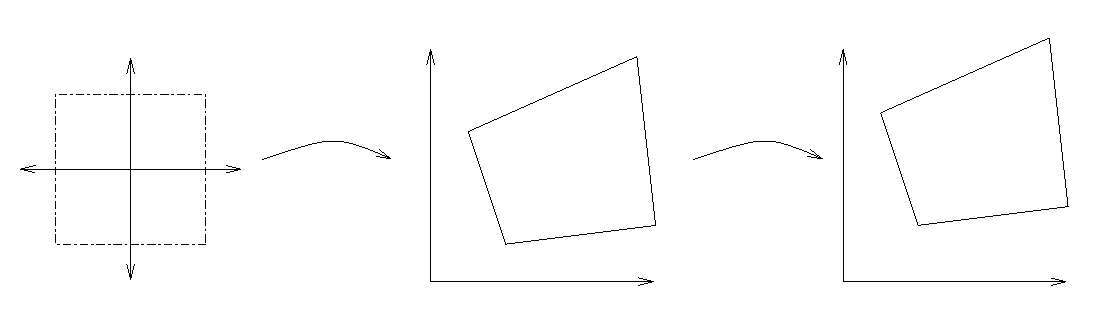
\includegraphics{isopml.ps}
\else
  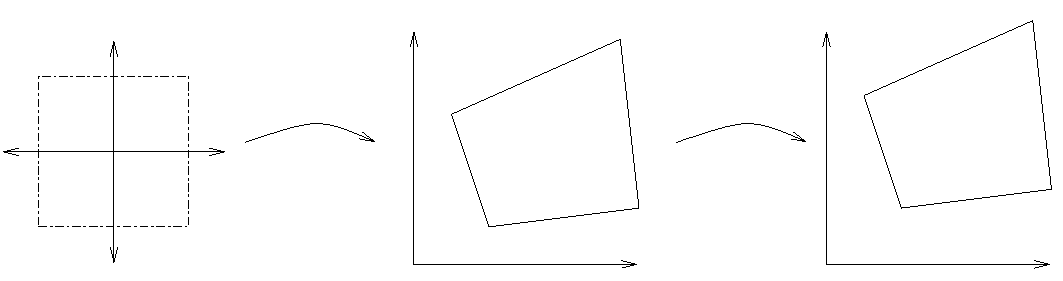
\includegraphics{isopml.pdf}
\fi
\end{picture}
\setlength{\unitlength}{3947sp}%
%
\begingroup\makeatletter\ifx\SetFigFont\undefined%
\gdef\SetFigFont#1#2#3#4#5{%
  \reset@font\fontsize{#1}{#2pt}%
  \fontfamily{#3}\fontseries{#4}\fontshape{#5}%
  \selectfont}%
\fi\endgroup%
\begin{picture}(8487,2239)(289,-1694)
\put(1051,314){\makebox(0,0)[lb]{\smash{{\SetFigFont{12}{14.4}{\familydefault}{\mddefault}{\updefault}{\color[rgb]{0,0,0}$\xi_2$}%
}}}}
\put(1951,-886){\makebox(0,0)[lb]{\smash{{\SetFigFont{12}{14.4}{\familydefault}{\mddefault}{\updefault}{\color[rgb]{0,0,0}$\xi_1$}%
}}}}
\put(5476,-1636){\makebox(0,0)[lb]{\smash{{\SetFigFont{12}{14.4}{\familydefault}{\mddefault}{\updefault}{\color[rgb]{0,0,0}$x_1$}%
}}}}
\put(3526,389){\makebox(0,0)[lb]{\smash{{\SetFigFont{12}{14.4}{\familydefault}{\mddefault}{\updefault}{\color[rgb]{0,0,0}$x_2$}%
}}}}
\put(6826,389){\makebox(0,0)[lb]{\smash{{\SetFigFont{12}{14.4}{\familydefault}{\mddefault}{\updefault}{\color[rgb]{0,0,0}$\tilde{x}_2$}%
}}}}
\put(8776,-1636){\makebox(0,0)[lb]{\smash{{\SetFigFont{12}{14.4}{\familydefault}{\mddefault}{\updefault}{\color[rgb]{0,0,0}$\tilde{x}_1$}%
}}}}
\put(4126,-961){\makebox(0,0)[lb]{\smash{{\SetFigFont{12}{14.4}{\familydefault}{\mddefault}{\updefault}{\color[rgb]{0,0,0}$\Omega^e$}%
}}}}
\put(7501,-886){\makebox(0,0)[lb]{\smash{{\SetFigFont{12}{14.4}{\familydefault}{\mddefault}{\updefault}{\color[rgb]{0,0,0}$\tilde{\Omega}^e$}%
}}}}
\put(676,-1111){\makebox(0,0)[lb]{\smash{{\SetFigFont{12}{14.4}{\familydefault}{\mddefault}{\updefault}{\color[rgb]{0,0,0}$\Omega^{\Box}$}%
}}}}
\put(6076,-211){\makebox(0,0)[lb]{\smash{{\SetFigFont{12}{14.4}{\familydefault}{\mddefault}{\updefault}{\color[rgb]{0,0,0}$\tilde{x}(x)$}%
}}}}
\put(2626,-211){\makebox(0,0)[lb]{\smash{{\SetFigFont{12}{14.4}{\familydefault}{\mddefault}{\updefault}{\color[rgb]{0,0,0}$x(\xi)$}%
}}}}
\end{picture}%
}
  \caption{Concatenated isoparametric mapping and PML coordinate mapping}
  \label{isopml-fig}
\end{figure}

To derive the weak form of the PML equation in the $x$ coordinate
(Equation \ref{weak-form-eq3}), we performed a change of variables
in the integrals of Equation \ref{weak-form-eq2}.  Because isoparametric
finite elements already use mapped integration, though, we can naturally
concatenate the change of variables associated with the PML mapping
into the change of variables associated with the isoparametric coordinate
transformation.

Consider the element in Figure~\ref{isopml-fig}.  Suppose we choose
shape functions $N_I$, so that the solution within the element has the
form $u = \sum_I N_I u_I$ and $w = \sum_I N_I w_I$.  Then the nodal submatrices
for the element stiffness and mass are given by
\begin{eqnarray}
  \label{stiffness-term}
  k^e_{IJ} & = &
    \int_{\Omega^{\Box}} \tilde{B}_I^T D \tilde{B}_J \tilde{J} d\Omega \\
  \label{mass-term}
  m^e_{IJ} & = &
    \left( \int_{\Omega^{\Box}} \rho N_I^T N_J \tilde{J} d\Omega \right) \bfI
\end{eqnarray}
where the nodal matrices $\tilde{B}_I$ come from transforming
coordinates in the standard $B$-matrix
formulation~\cite{Zienkiewicz:2000:FEMa}, $D$ is the standard matrix
of material parameters, and $\tilde{J}$ is the Jacobian of the
composition of the PML mapping with the isoparametric mapping:
\begin{equation}
  \tilde{J} = 
    \det\left( \frac{\partial x}{\partial \xi} \right)
    \det\left( \Lambda \right)
\end{equation}
In practice, we evaluate the integrals numerically by Gaussian
quadrature in the parent domain.  Whether the quadrature is done
analytically or numerically, the form of the integrands in
(\ref{stiffness-term}) and (\ref{mass-term}) guarantees that the
mass and stiffness matrices will be complex symmetric.

We note in passing that this interpretation of the PML in terms of an
additional coordinate transformation works with plane stress, plane
strain, axisymmetric, or three-dimensional problems.  In the
axisymmetric case, however, the factor of $r$ that appears in the
integrands should \emph{not} be transformed into the PML coordinate
systems, since that factor of $r$ comes from the Jacobian of the
mapping to the $(r,z)$ coordinates, and not from the mapping to the
$(\tilde{r}, \tilde{z})$ coordinates.
\note{Do I want to spell this out in more detail?}

For many problems, a reasonable choice of coordinate transformations
is to independently stretch each coordinate $x_i$, so that $\Lambda$
is a diagonal matrix.  If we further choose stretching functions so
that $\Lambda$ can be described by low-order polynomials, then it
makes sense to use isoparametric interpolation to compute the values
of the stretching function.  That is, given values for $\lambda_1$ and
$\lambda_2$ at each node, we compute $\Lambda = \diag(\lambda_1,
\lambda_2)$ by interpolation at the Gauss points where it is
evaluated.


\section{Mode calculations, model reduction, and $Q$}

Though $Q$ is formally defined according to Equation (\ref{Q-def}) as
the ratio of the stored energy to the energy loss per radian, it is
more convenient to compute it in other ways.  If 
$\omega = \omega_0 + i \alpha$ is the complex-valued resonant frequency 
in radians/s, then~\cite{Senturia:2001:MD}
\begin{equation}
  Q = \frac{\omega_0}{2 \alpha}
\end{equation}
Experimentally, $Q$ can also be estimated as
\begin{equation}
  Q = \frac{\omega_0}{b}
\end{equation}
where $b$ is the bandwidth of frequencies where the response amplitude
is within $3$ decibels of the peak amplitude.

As we noted at the end of Section~\ref{elastic-pml-section}, the PML
coordinate transformations suggested in~\cite{Basu:2003:PML} are
dependent on the frequency, so that the attenuation through the PML
layer will be independent of the forcing frequency.  Using such a
frequency-dependent coordinate transformation, the complex resonant
frequencies $\omega$ will correspond to solutions to the nonlinear
eigenvalue problem $\det(\Kdynamic(\omega)) = 0$, where
\begin{equation}
  \Kdynamic(\omega) := K(\omega) - \omega^2 M(\omega).
\end{equation}
When the frequency range of interest is not too wide, though, the
parameters of the coordinate transformation may be chosen once to give
acceptable attenuation over the desired range, so that the approximate
dynamic stiffness for $\omega$ near a fixed reference frequency
$\omega_0$ is
\begin{equation}
  \Kdynamic^0(\omega) := K(\omega_0) - \omega^2 M(\omega_0).
\end{equation}
Finding roots such that $\det(\Kdynamic^0(\omega)) = 0$ is a linear
(generalized) eigenvalue problem, which we can now approach using
standard tools.

To find the damped eigenvalues near some specified reference frequency
$\omega_0$, we use a shift-and-invert Arnoldi procedure, described
in standard references on numerical linear 
algebra~\cite{Golub:1989:MC, Demmel:1997:ANL}.  This procedure computes
an orthonormal basis $V$ for the Krylov subspace
\begin{equation}
  \calK_n(\Kdynamic(\omega_0), x_0) = 
    \sspan\{ u_0, \Kdynamic^0(\omega_0)^{-1} u_0, \ldots,
                  \Kdynamic^0(\omega_0)^{-(n-1)} u_0 \};
\end{equation}
the characteristic damped frequencies are then approximated by the
eigenvalues of $V^H \Kdynamic^0(\omega) V$.  For computing a few
isolated eigenvalues near $\omega_0$, the main cost of the
shift-and-invert Arnoldi procedure is to compute the factorization
needed to apply $\Kdynamic^0(\omega_0)$.  In our numerical
experiments, we use UMFPACK~\cite{Davis:2004:AUU} to factor the
shifted matrix, and we use \texttt{eigs}, MATLAB's interface to the
implicitly-restarted Arnoldi code ARPACK~\cite{Lehoucq:1998:AUG}, to
compute the desired eigenvalues.

Though damped mode calculations are illuminating, they do not give a
complete picture of the frequency response behavior.  In practice, we
are interested in systems in which there is a single
periodically-forced input and a single output determined by some
sensed displacement.  Suppose $F$ is a time-harmonic load vector, and
the output is a linear function of displacement $P^T u$.
Then we are really interested in computing the transfer function
\begin{equation}
  H(\omega) = P^T \Kdynamic(\omega)^{-1} F
\end{equation}
which we approximate for a range of frequencies near $\omega_0$ by
\begin{equation}
  H^0(\omega) = P^T \Kdynamic^0(\omega)^{-1} F.
\end{equation}  
Even if $\Kdynamic^0(\omega)$ is nearly singular at some frequency,
the response amplitude $|H^0(\omega)|$ may not peak, since $F$ may be
nearly orthogonal to the forcing that drives the mode, or $P$
orthogonal to the modal displacement pattern.  Therefore, we would
like to examine $H^0(\omega)$ directly using a Bode plot.

Since the dimension $N$ of $\Kdynamic^0(\omega)$ is large, it is
expensive to evaluate $H^0(\omega)$ directly.  Instead, we construct
a \emph{reduced-order model} of dimension $n \ll N$, which we use to
approximate $H^0(\omega)$.  Krylov-subspace projections, like the
Arnoldi projection we used to compute damped frequencies, are often
used to build reduced models of large
systems~\cite{Bai:2002:KST,Antoulas:2001:ALS}.  If we build an
orthogonal basis $V$ for a small Krylov subspace using
shift-and-invert Arnoldi, then we can approximate $H^0(\omega)$ near the
shift $\omega_0$ by
\begin{equation}
  \hat{H}^0(\omega) := (V^H P)^H (V^H \Kdynamic^0(\omega) V)^{-1} (V^H F).
\end{equation}

Though $\hat{H}^0(\omega)$ is often a good approximation to
$H^0(\omega)$, the projected system matrix $V^H \Kdynamic^0(\omega) V$
does not preserve the complex symmetric structure of the original
discretization.  We can construct a symmetry-preserving reduced-order
model by choosing an orthonormal projection basis $W$ such that
\begin{equation}
  \sspan(W) = \sspan([\Re(V), \Im(V)]).
\end{equation}
The resulting reduced model will have at least the same level of
accuracy as the usual Arnoldi projection, but will maintain the
complex symmetry of the original system matrices.  Also, because $W$
is a real-valued basis, projection onto the space spanned by $W$
corresponds to a Bubnov-Galerkin discretization of the PML equation
with shape functions $N_I^\mathrm{reduced} = \sum_J W_{IJ} N_J$.


\section{Study of a disk resonator}

\subsection{Disk resonator design}

\begin{figure}
  \begin{center}
    \scalebox{0.5}{\begin{picture}(0,0)
\ifx\pdfoutput\undefined
  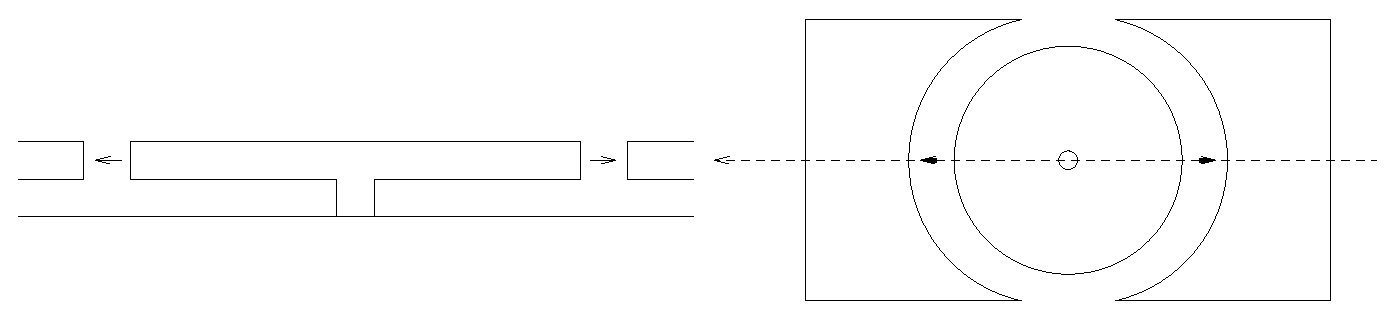
\includegraphics{michmodel.ps}
\else
  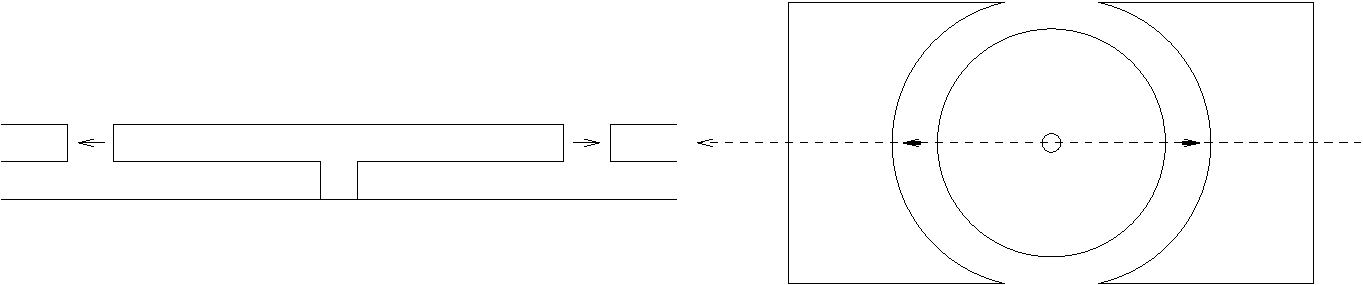
\includegraphics{michmodel.pdf}
\fi
\end{picture}
\setlength{\unitlength}{3947sp}%
%
\begingroup\makeatletter\ifx\SetFigFont\undefined%
\gdef\SetFigFont#1#2#3#4#5{%
  \reset@font\fontsize{#1}{#2pt}%
  \fontfamily{#3}\fontseries{#4}\fontshape{#5}%
  \selectfont}%
\fi\endgroup%
\begin{picture}(10899,2274)(289,-1498)
\put(2701,-61){\makebox(0,0)[lb]{\smash{{\SetFigFont{12}{14.4}{\familydefault}{\mddefault}{\updefault}{\color[rgb]{0,0,0}Disk}%
}}}}
\put(376,-61){\makebox(0,0)[lb]{\smash{{\SetFigFont{12}{14.4}{\familydefault}{\mddefault}{\updefault}{\color[rgb]{0,0,0}Electrode}%
}}}}
\put(2776,-1036){\makebox(0,0)[lb]{\smash{{\SetFigFont{12}{14.4}{\familydefault}{\mddefault}{\updefault}{\color[rgb]{0,0,0}Wafer}%
}}}}
\put(6901,-1186){\makebox(0,0)[lb]{\smash{{\SetFigFont{12}{14.4}{\familydefault}{\mddefault}{\updefault}{\color[rgb]{0,0,0}$V_+$}%
}}}}
\put(8626,-811){\makebox(0,0)[lb]{\smash{{\SetFigFont{12}{14.4}{\familydefault}{\mddefault}{\updefault}{\color[rgb]{0,0,0}$V_-$}%
}}}}
\put(9976,-1186){\makebox(0,0)[lb]{\smash{{\SetFigFont{12}{14.4}{\familydefault}{\mddefault}{\updefault}{\color[rgb]{0,0,0}$V_+$}%
}}}}
\end{picture}%
}
  \end{center}
  \caption{Schematic of the Michigan disk resonator.  An overhead view
           (right) shows the arrangement of the resonating disk and
           the electrodes which force it.  An idealized cross-section (left)
           is used in an axisymmetric simulation, where the wafer substrate
           is treated as semi-infinite using a perfectly-matched layer.}
  \label{michfig}
\end{figure}

As an example application of the perfectly matched layer technology,
we study the loss of energy through the anchor in a family of
disk-shaped MEMS resonators~\cite{Wang:2003:SAG,Wang:2004:GND}.  A
schematic of the device is shown in Figure~\ref{michfig}.  A thin
polysilicon disk is supported on a polysilicon post above the
substrate stack.  The disk is surrounded by drive electrodes, and the
potential difference between the disk and the drive electrodes pulls
the disk radially outward at the rim.  The disk is driven near the
frequency of the first or second axisymmetric, radial, in-plane mode.
In~\cite{Wang:2003:SAG}, the disk is made of polysilicon;
\cite{Wang:2004:GND} describes both both polysilicon and polydiamond disk.

A major source of energy loss in this device is the propagation of
elastic waves down the supporting post and into the wafer below, where
they are largely dissipated.  Relative to the size of the resonating
device, the wafer is very large.  We assume that the wafer is
effectively infinite in extent, so that none of the waves that radiate
into the substrate will be reflected.  We use a perfectly matched
layer to model the wafer as a semi-infinite half space.

In the actual device, there are silicon nitride and silicon oxide
films between the device (which is made of polysilicon) and the wafer
(which is made of single crystal silicon).  In our model, the same
material properties (those of polysilicon) are used for both the
resonator and the underlying wafer.  Consequently, our model ignores
material interfaces which occur in the actual device and which might
reflect energy back.  We therefore expect that our model will
overestimate the losses at resonance (and therefore underestimate the
quality factor $Q$).  Note that this is a simplification in the model,
not an inherent limitation of the PML technology; indeed, one of the
attractions of PMLs is the ability to handle layered media.

Besides the simplified substrate stack model, there are several other
possible sources of error.  When the device is made of a single
material, the predicted $Q$ (but not the real part of the frequency)
is independent of Young's modulus; however, if the ratios between the
material properties in a silicon-diamond device are inaccurate, $Q$
might be affected.  Also, in~\cite{Wang:2003:SAG,Wang:2004:GND}, the
post extends substantially above the disk, because for alignment
purposes, the post is built by filling a hole through the disk.  We
completely ignore the complexities of the post geometry in our model.
Also, the fabricated geometry may not perfectly match the designed
geometry.


\subsection{Convergence of $Q$}

\begin{figure}
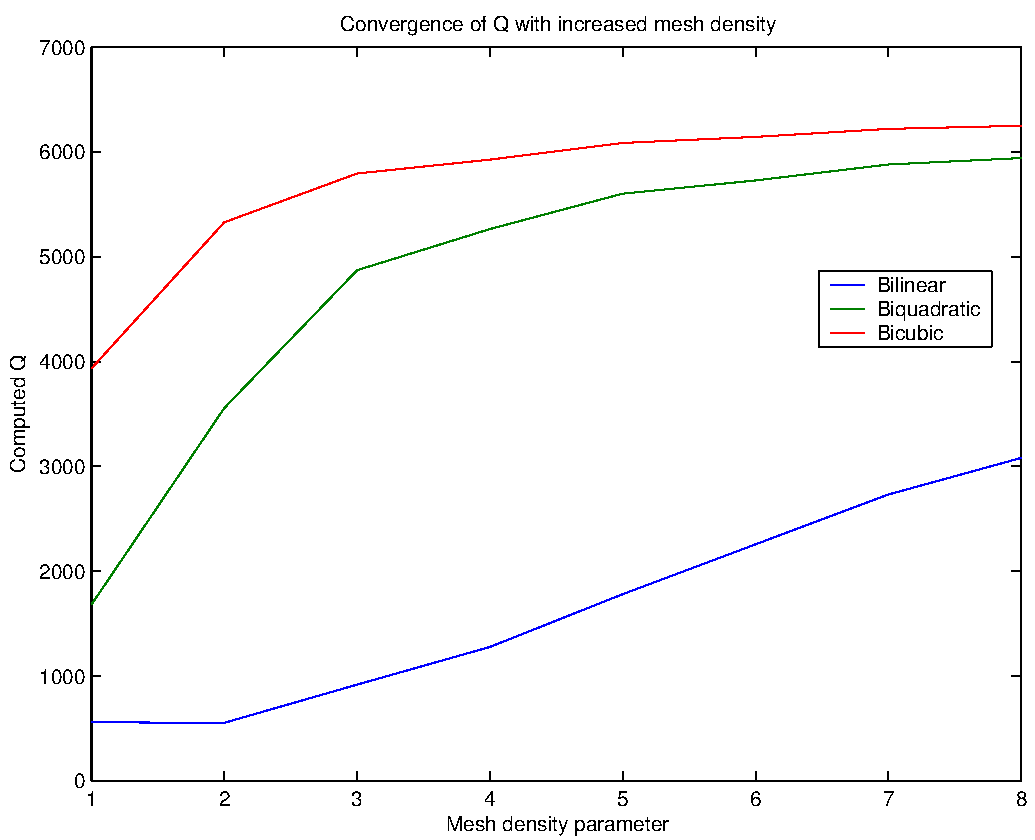
\includegraphics[height=2.8in]{Qconverge.pdf}
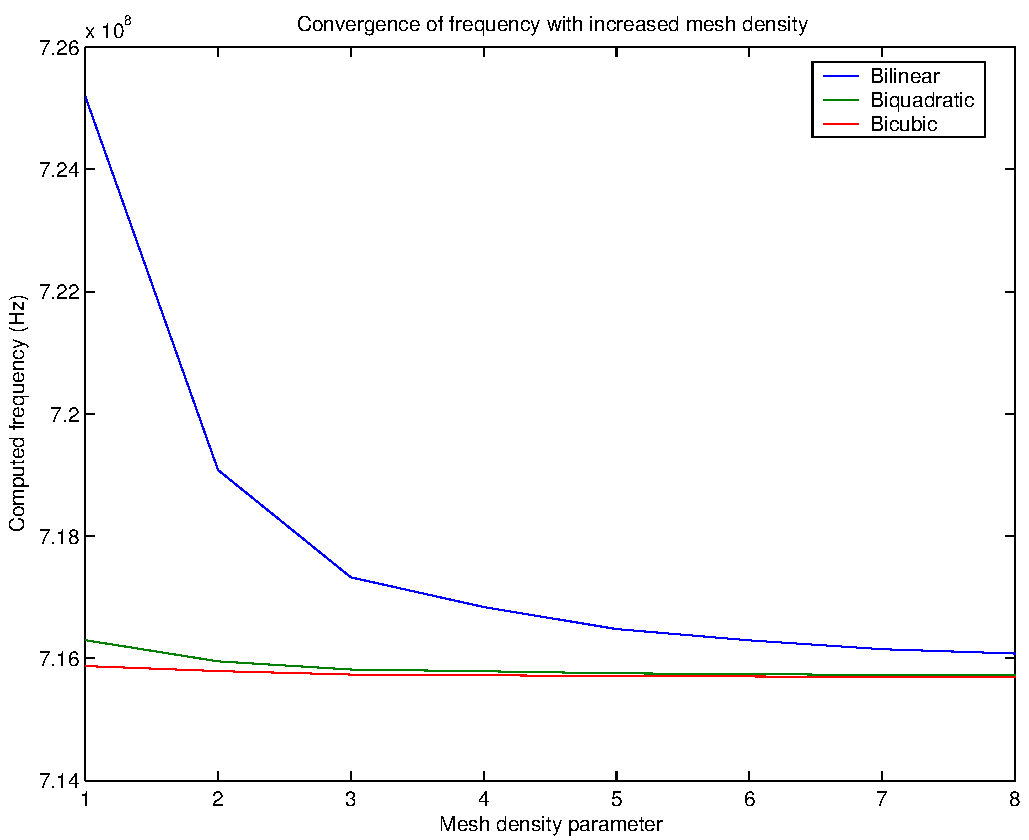
\includegraphics[height=2.8in]{wconverge.pdf}
\caption{Convergence of $Q$ and $\omega_\mathrm{center}$ for the second
         radial mode of the Michigan disk.}
\label{converge-fig}
\end{figure}

We first consider the polysilicon disk resonator described
in~\cite{Wang:2003:SAG}, which has a disk $20$ \um\ in diameeter
and $2$ \um\ thick, supported $0.5$ \um\ above the substrate
by a post $2$ \um in diameter.
For the second radial mode, the measured $Q$ for the actual device was
7330 in vacuum and 6100 in air, and the center frequency was 733 MHz.
In our best-resolved simulation, we computed a $Q$ value of 6250 at a
center frequency of 715.6 MHz.  Perhaps surprisingly, relatively fine
resolution was required to obtain convergence.  When the mesh was
under-resolved, the $Q$ factor was drastically underestimated,
possibly because the very small flux reaching the anchor base could
not be resolved by the mesh, and was therefore overestimated.
\note{This isn't a very satisfying analysis.  Can I say something a bit
  more quantitative?  Will under-resolved meshes always result in low
  estimates of $Q$?  Can I get away with refining the mesh in the
  vicinity of the corner and leaving the rest mostly alone?}  
We computed the value of $Q$ using both linear and higher-order
elements at several mesh densities (Figure \ref{converge-fig}).  For a
given mesh density parameter $m$, we chose elements so that nodes were
as near as possible to $1/m$ microns apart.  We computed $Q$ and
$\omega_\mathrm{center}$ by using shift-and-invert Arnoldi with an
initial shift of 715 MHz to find the damped eigenvalue.  The Arnoldi
iteration converged very rapidly, and most of the time was spent in
the LU factorization of the shifted matrix.
\note{Question from Jim: does this have the right asymptotic convergence?}

\subsection{Observed energy loss mechanism}


\begin{figure}
\begin{center}
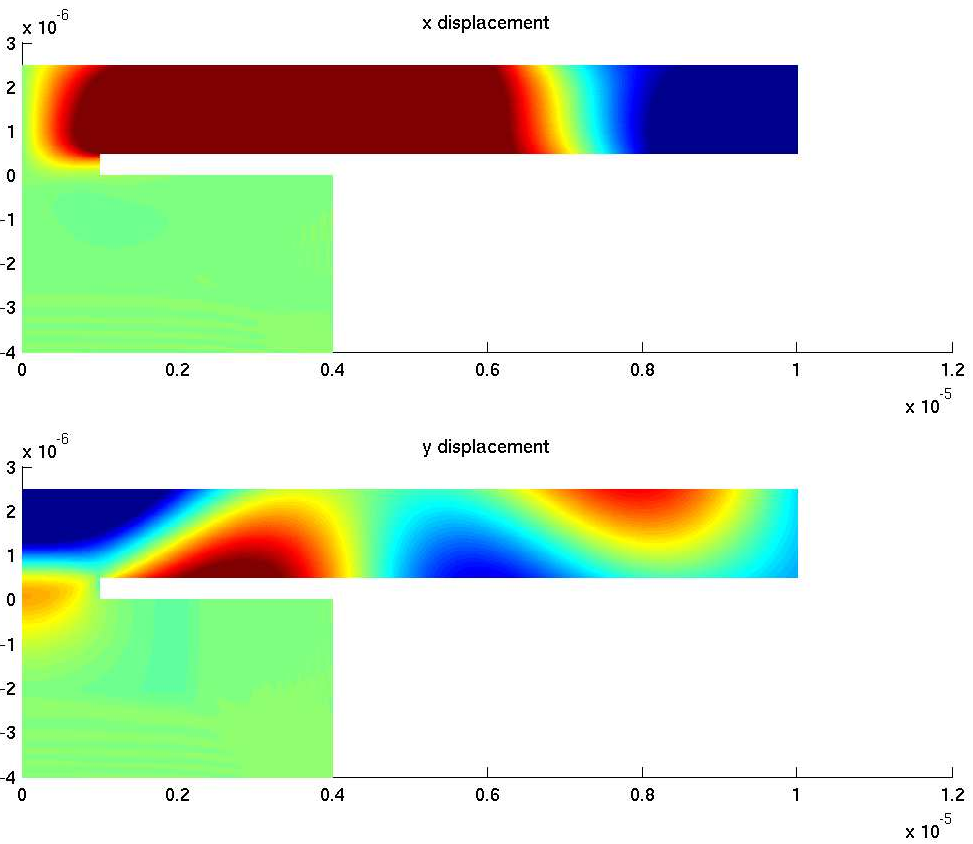
\includegraphics[height=3in]{drive715.pdf}
\end{center}
\caption{Forced displacement (real part) for the disk resonator
         model at 715 MHz}
\label{forced-mode-fig}
\end{figure}

\begin{figure}
\begin{center}
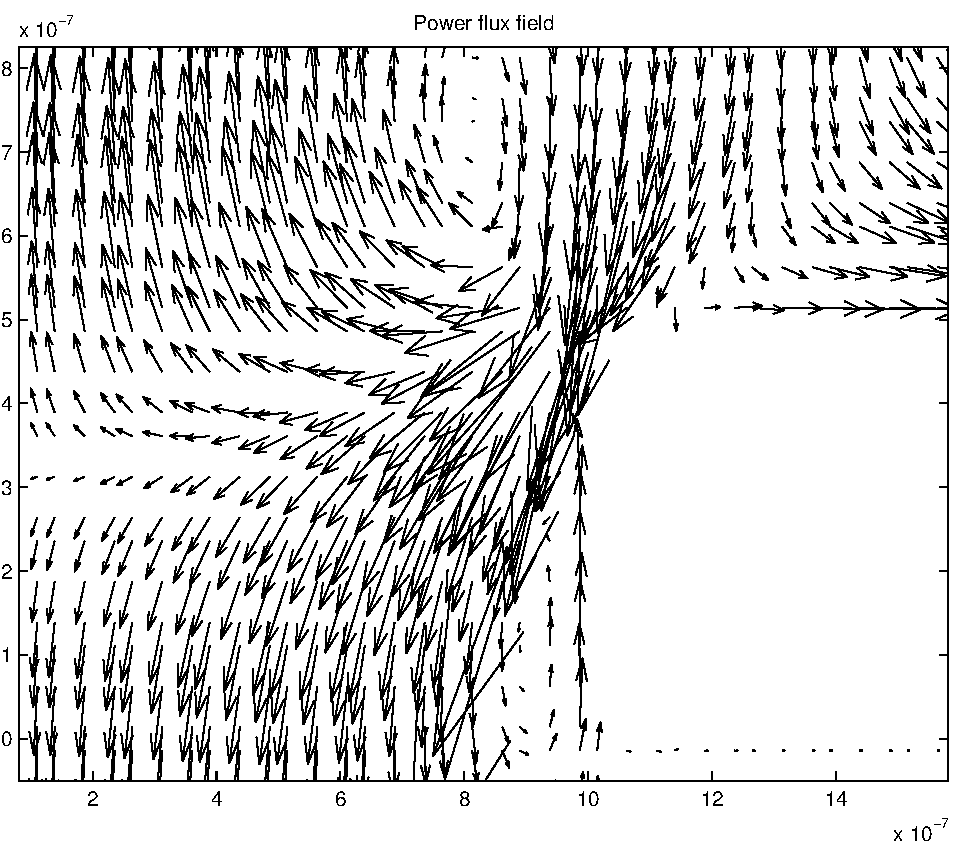
\includegraphics[height=3in]{power715a.pdf}
\end{center}
\caption{Time-averaged energy flux vector field in the disk
         resonator driven at 715 MHz.  This plot shows only the
         region in the vicinity of the post.}
\label{forced-flux-fig}
\end{figure}

Figure~\ref{forced-mode-fig} shows the behavior of the disk when
driven at 715 MHz, just slightly below the resonant frequency.  The
amplitudes of both the radial and vertical displacements are shown at
the point when the forcing is maximal.  The majority of the
displacement occurs in the disk itself, but there is some motion in
the post as well.  Though the forcing is in the radial direction, the
Poisson effect leads to motion in the vertical direction as well.  At
the center of the disk, the motion is entirely vertical, and this
vertical ``pump'' motion results in displacement waves that travel
down the post and into the substrate.  In an animation, it is possible
to see low-amplitude waves radiating away from the post to be absorbed
into the perfectly matched layer.
\note{Is it possible to estimate losses in this case through some
  sort of perturbation analysis?}

To get a better understanding of the behavior shown in 
Figure~\ref{forced-mode-fig}, we compute the energy density flux:
\begin{equation}
  F(t) = -\Re( \sigma e^{i \omega t} ) 
          \Re( v e^{i \omega t} )
\end{equation}
where $\sigma$ is the stress tensor and $v$ is the velocity vector.
Since the energy flux changes over time, we time-average to obtain
the mean energy density flux:
\begin{equation}
  \bar{F} = -\Re( \sigma v^* )
\end{equation}
where $v^*$ is the complex conjugate of the velocity.  For a standing
wave, the displacement and stress are pure real, and $v = iku$ is pure
imaginary, so there is no mean energy flux.  Therefore, the mean energy
flux field tells us something about the departure from the standing-wave
behavior that occurs in a lossless system.  Figure~\ref{forced-flux-fig}
shows the mean energy flux for a region of the resonator near the
edge of the post.  The flux vectors in the body of the disk form cycles
which carry energy around inside the disk, but do not let it escape into
the substrate.  Near the post, however, the cycle pattern is broken, and
the energy flux plot shows a ``spray'' of energy that travels down the
post and into the substrate.

\subsection{Mode mixing in the disk resonator}

% Geometric sensitivity
% Root locus plot
% Forced response shapes
% Non-normality measure and effects of non-normality
% Model reduction

Because surface micromachining is often imprecise, it is important
to understand the sensitivity of resonator designs to variations
from the nominal geometry and material parameters.  A study of the effect
of varying film thickness on the $Q$ value predicted by the resonator
illustrates the need for such understanding, and also the need for
simulation tools capable of teasing out subtleties that cannot easily
be predicted by hand models.

\begin{figure}
  \label{Q-locus-plot}
  \begin{center}
    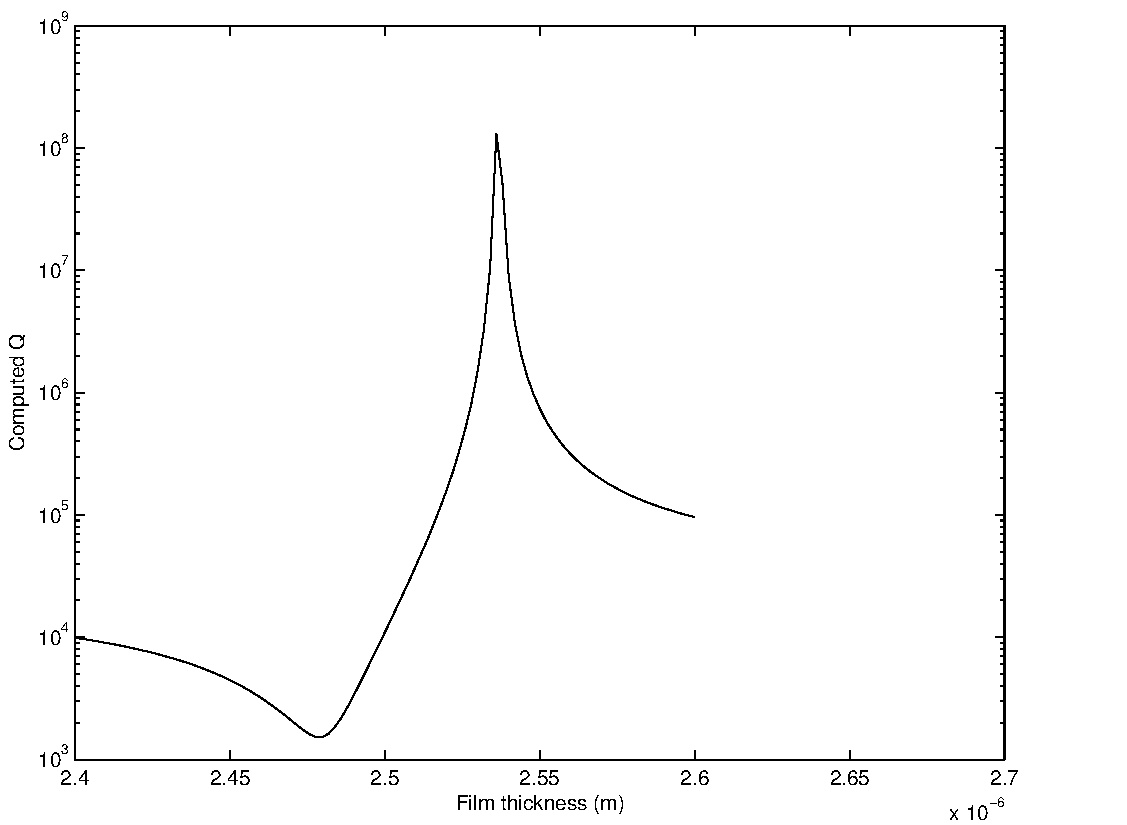
\includegraphics[height=3in]{Qmain1.pdf}
    \caption{$Q$ as a function of film thickness}
  \end{center}
\end{figure}

\begin{figure}
  \label{cos-theta-plot}
  \begin{center}
    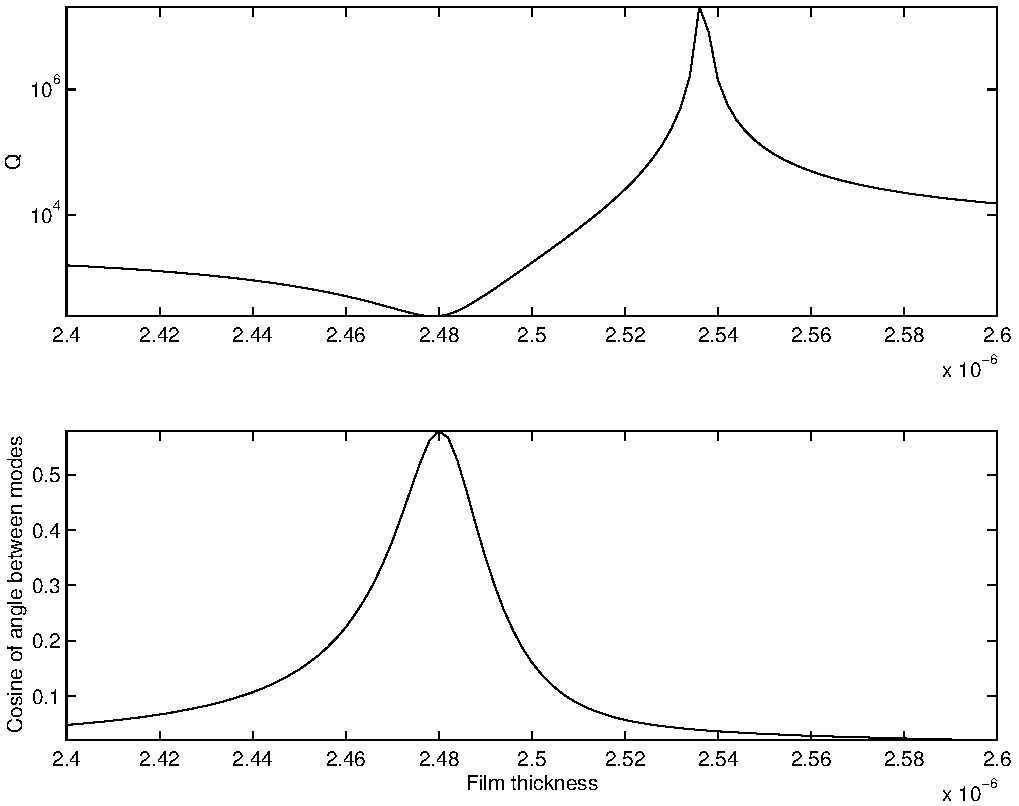
\includegraphics[height=3in]{theta_plot.pdf}
    \caption{Effect of mode mixing.  The angle between the radial
             and bending modes is measured according
             to the mass-weighted $L^2$ inner product over the
             untransformed part of the domain.  Note that damping
             is maximized where the angle between the modes is smallest.}
  \end{center}
\end{figure}

\begin{figure}
  \label{root-locus-plot}
  \begin{center}
    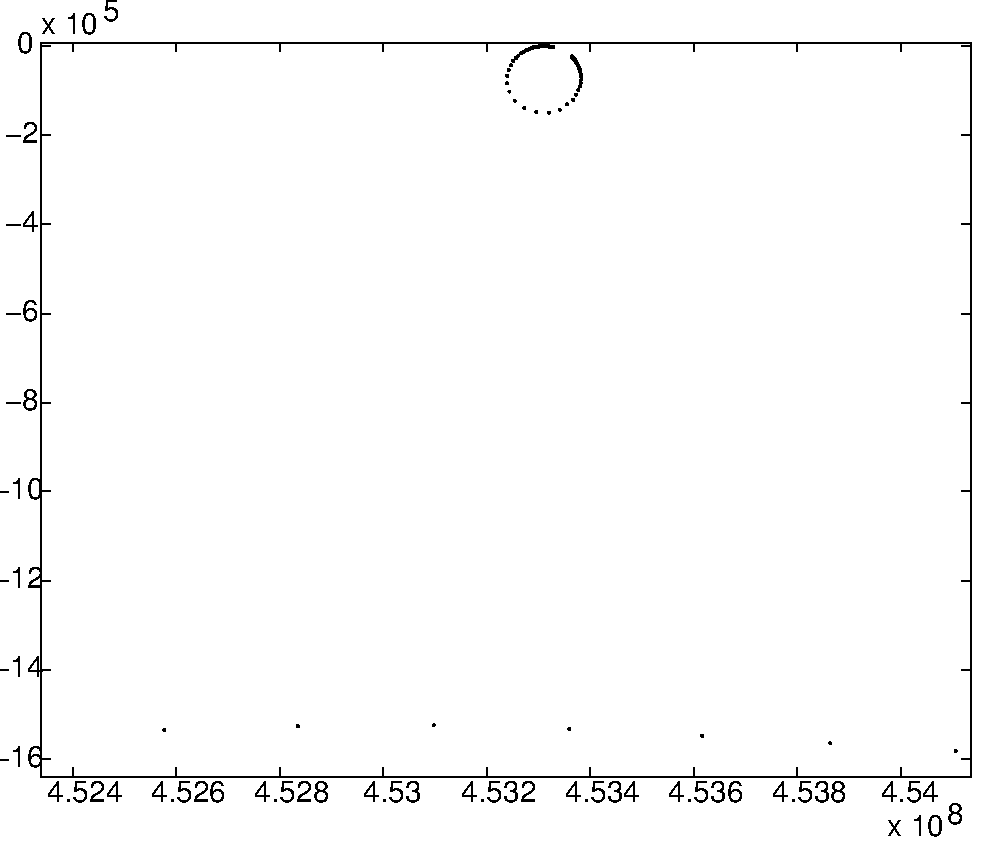
\includegraphics[height=3in]{rootlocus4.pdf}
    \caption{Eigenvalue mixing near critical film thickness}
  \end{center}
\end{figure}

Figure~\ref{Q-locus-plot} shows the variation of $Q$ as a function of
film thickness.  The disk is made of polydiamond, the post is made of
polysilicon, and the device is driven in the first radial mode.  For
film thicknesses near 2.5~\um, the computed $Q$ varies rapidly over
nearly five orders of magnitude.  Though at first we believed this
might be an artifact of the discretization, varying the size of the
PML region and the parameters in the PML transformation did not
substantially affect the behavior.  On more careful investigation, we
saw that the sharp change in $Q$ appeared when the radial mode nearly
coincided in frequency with one of the bending modes.
Figure~\ref{root-locus-plot} shows part of a root-locus plot showing
the curves traced out by the two eigenvalues nearest the target
frequency as the film thickness in the model is varied.  The top curve
is the path of the eigenvalue corresponding to the radial mode; the
bottom curve is the path of the eigenvalues corresponding to the
bending mode.  As the two mode frequencies approach each other, the
radial mode frequency swings in a circle, first away from the real
axis, then back toward it, then back out again.  A visualization of
the forced response shows the picture more clearly: for film
thicknesses that yield very low $Q$, the radial forcing excites a
mixture of radial extension and bending which causes large amplitude
displacement waves to be excited at the post; while for film
thicknesses where $Q$ is high, the radial motion and the bending motion
interact in such a way that almost no motion occurs at the post.

\begin{figure}
  \label{disk-bode}
  \begin{center}
    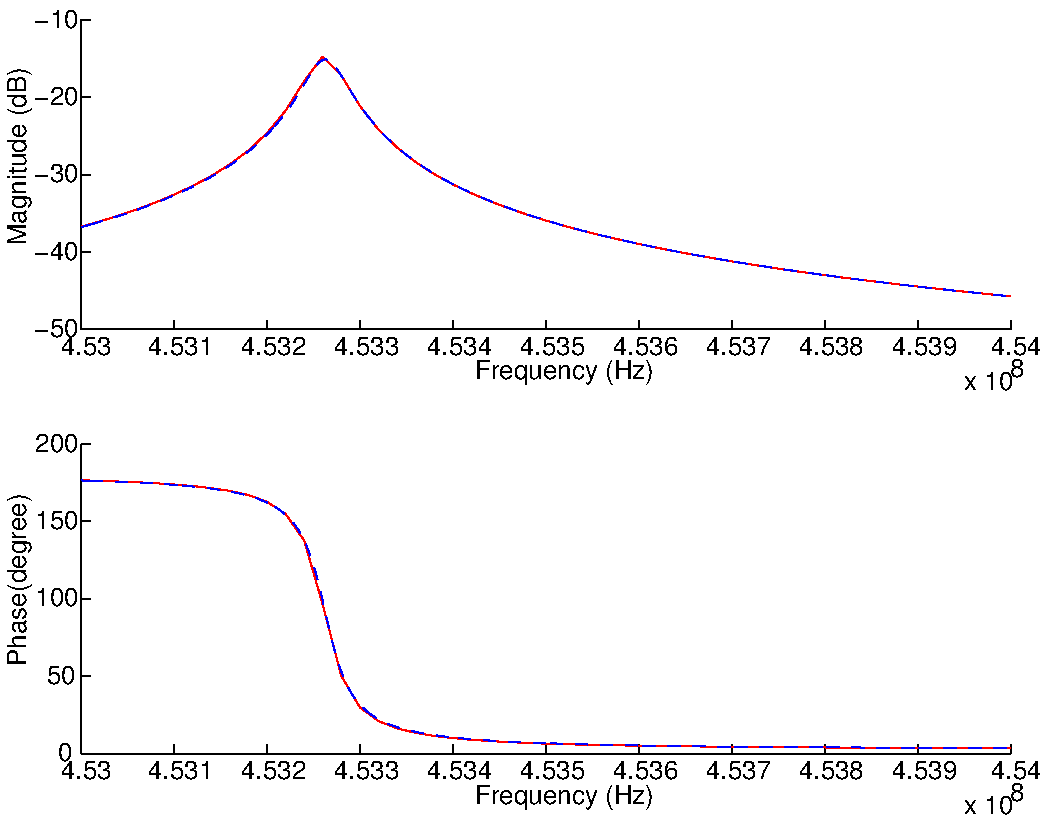
\includegraphics[height=3in]{rombode1.pdf}
    \caption{Bode plot for a disk resonator (exact and reduced)}
  \end{center}
\end{figure}

The bending mode significantly affects the radial peak, but not in a
way that is immediately obvious from a Bode plot.  Because the quality
of resonance of the bending mode is relatively low, and because
bending motion results in little displacement in the sense direction,
the peak for the bending motion is hidden by the much stronger peak
for the radial motion.  Suppose we compute a shift drawn from the hand
estimate for the disk frequency:
\begin{equation}
  \omega_\mathrm{shift} = 2.405 c/R,
\end{equation}
where $R$ is the disk radius and $c$ is the compression-wave velocity
in the disk material.  With this shift, we require only two steps of
shift-and-invert Arnoldi to resolve the two-dimensional invariant
subspace for both eigenvalues.  Projecting onto this subspace gives us
a local reduced-order model with a Bode plot which is indistinguishable
from the Bode plot of the first model (Figure~\ref{disk-bode}).

\bibliographystyle{plain}
\bibliography{dsbdoc}

\end{document}
